\documentclass[12pt,a4paper]{article}
\usepackage{../riemlabm}
\title{Induced EMF}
\lfoot{Regional Institute of Education Mysore}
\lhead{Induced EMF}
\chead{}
\rhead{Semester 6}
\cfoot{}
\rfoot{Physics}
\pagestyle{fancy}  

\begin{document} 
	\maketitle
	\section{OBJECTIVE}
		To study the emf induced in a circular coil as a function of the amplitude and time period of the magnet.
		
	\section{REQUIREMENTS}
		Circular coil, resistor, diode, capacitor, voltmeter, milliammeter, key
		
	\section{INTRODUCTION}
		
		Whenever the magnetic flux $\phi$ around a conductor changes, an emf is induced inside the conductor. This is known as \textit{Faraday's first law of electromagnetic induction.} 
		
		This experiment works on the principle of electromagnetic induction.
		
		$$\varepsilon=-\dfrac{d\theta}{dt}$$
	\section{PROCEDURE}
		\begin{figure}[!htb]
			\centering
			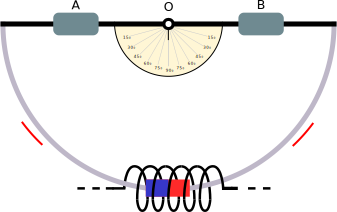
\includegraphics[scale=1]{emf-setup.pdf}
			\caption{Experimental setup}
		\end{figure}
		
		\subsection{Potential difference versus amplitude}
		
		\begin{enumerate}
			\item The apparatus is set up as shown in figure 1. The magnet is placed on the circular arc and is allowed to oscillate through the coil by releasing it through different angles.
			
			\item Connect the coil in the above apparatus as shown in the circuit diagram in figure 2.
			
			\begin{figure}[!htb]
				\centering
				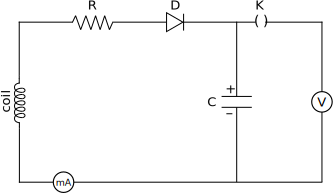
\includegraphics[scale=1]{emf-circuit.pdf}
				\caption{Circuit diagram}
			\end{figure}
			
			\item Short the terminals of the capacitor in order to discharge it completely. 
			
			\item Keep the masses at equal distances from the pivot.
			
			\item Set the semicircular arc into oscillations by releasing it from a known amplitude of, say, $15\degree$.
			
			\item When the induced emf charges the capacitor to its maximum, the galvanometer deflection becomes zero and steady. Note down the potential difference across the capacitor at this stage. This gives a measure of the induced emf.
			
			\item The terminals of the capacitor is again shorted, bringing its potential difference to zero.
			
			\item Repeat this process for different amplitudes of oscillations (say $20\degree,\ 25\degree,\ 30\degree,\ 35\degree,\ $etc.)
			
			\item Plot a graph of potential difference ($\varepsilon$) against amplitude of oscillation ($\theta$).
		\end{enumerate}
		
		\subsection{Emf versus time period}
			
			\begin{enumerate}
				\item Measure the separation of the masses OA and OB from the pivot.
				
				\item Oscillate the arc by a constant amplitude of, say, $20\degree$.
				
				\item Measure the time taken for 10 oscillations and hence find the time period $T$ of the oscillating arc.
				
				\item Again, the potential difference is measured when the galvanometer attains steady state.
				
				\item Now change the length of separation OA and OB by equal amounts so that the balance is maintained.
				
				\item Repeat the experiment for different lengths of separations, keeping the amplitude constant, i.e., $20\degree$.
				
				\item Plot a curve of emf ($\varepsilon$) versus time period ($T$).
			\end{enumerate}
			
			\section{OBSERVATIONS}
			\subsection{Potential difference versus amplitude}
			\begin{center}
				\begin{tabular}{|c|c|>{\centering\arraybackslash}p{45pt}|>{\centering\arraybackslash}p{45pt}|>{\centering\arraybackslash}p{45pt}|c|}
				\hline
				\rowcolor{b1!50}No.&	Amplitude&	\multicolumn{3}{c|}{Potential difference}&	Mean $\varepsilon$\\ 
				
				\rowcolor{b1!50}&	of oscillations $\theta (\degree)$& \multicolumn{3}{c|}{across capacitor ($V$)}&	($V$)\\ \cline{3-5}
				
				\rowcolor{b1!50}&& $\varepsilon_{1}$& $\varepsilon_{2}$& $\varepsilon_{3}$& \\ \hline
				
				1&20&&&& \\ \hline
				2&25&&&& \\ \hline
				3&30&&&& \\ \hline
				4&35&&&& \\ \hline
				5&40&&&& \\ \hline
			\end{tabular}
			\end{center}
			
			\subsection{Emf versus time period}
			Amplitude of oscillations $= \rule{10ex}{0.2pt}$\\
			No. of oscillations $= \rule{10ex}{0.2pt}$
			\begin{center}
				\begin{tabular}{|>{\centering\arraybackslash}p{30pt}|>{\centering\arraybackslash}p{30pt}|>{\centering\arraybackslash}p{45pt}|>{\centering\arraybackslash}p{45pt}|c|c|>{\centering\arraybackslash}p{45pt}|>{\centering\arraybackslash}p{45pt}|c|c|}
					\hline
					\rowcolor{b1!50}\multicolumn{2}{|c|}{Distance}& \multicolumn{2}{c|}{Time taken}& Mean& Time& \multicolumn{2}{c|}{Potential difference}& Mean& $\frac{1}{T}$\\ 
					
					\rowcolor{b1!50}\multicolumn{2}{|c|}{(cm)}& \multicolumn{2}{c|}{for 5 oscillations (s)}& $t$ (s)& period $T$ (s)& \multicolumn{2}{c|}{across capacitor (V)}& $\varepsilon$ (V)& (s$^{-1}$)\\ \cline{1-2} \cline{3-4} \cline{7-8}
					
					\rowcolor{b1!50}OA& OB& $t_1$& $t_2$& & & $\varepsilon_1$& $\varepsilon_2$& & \\ \hline
					
					&&&&&&&&& \\ \hline
					&&&&&&&&& \\ \hline
					&&&&&&&&& \\ \hline
					&&&&&&&&& \\ \hline
					&&&&&&&&& \\ \hline
				\end{tabular}
			\end{center}
			
			\section{CALCULATIONS}
				From the table in section 5.1, plot a curve of potential difference against the amplitude of oscillations, to get a straight line (figure 3).
				
				\begin{figure}[!htb]
					\centering
					\includegraphics{E-v-theta.png}
					\caption{}
				\end{figure}	
				
				From the table in 5.2, plot a curve of the EMF versus the time period of oscillations ($T$) to get a straight line with a negative slope:
				
				\begin{figure}[!htb]
					\centering
					\includegraphics{E-v-T.png}
					\caption{}
				\end{figure}
				
				\section{RESULT}	
				
				The emf induced was studied as a function of the amplitude and time period of oscillations of the magnet. 	
\end{document}